% !TEX program = lualatex
\documentclass[11pt]{article}

% -------- LuaLaTeX : polices et langue --------
\usepackage{fontspec}
\setmainfont{Latin Modern Roman}
\setsansfont{Tex Gyre Heros}
%\renewcommand{\familydefault}{\sfdefault} % force le sans serif par défaut
\usepackage{polyglossia}
\setdefaultlanguage{french}

% -------- Mise en page --------
\usepackage[a4paper,margin=1cm]{geometry}
\usepackage{multicol}
\usepackage{fancyhdr}
\pagestyle{empty}
\usepackage[most]{tcolorbox}

% -------- Mathématiques --------
\usepackage{amsmath,amssymb,mathtools}
\usepackage{icomma}
% \sisetup{locale=FR}

\usepackage{enumitem}
\setlist[itemize]{left=0pt}
\setlist[enumerate]{left=0pt, label=\textbf{\arabic*}.}

\usepackage{ProfCollege}
\usepackage{ProfMaquette}

\usepackage{tabularray}

% -------- Divers --------
\setlength{\parindent}{0pt}

\begin{document}

\begin{multicols}{2}

    \begin{Maquette}[Fiche]{Theme=Calcul littéral, Niveau=Quatrième}

        \begin{exercice}
            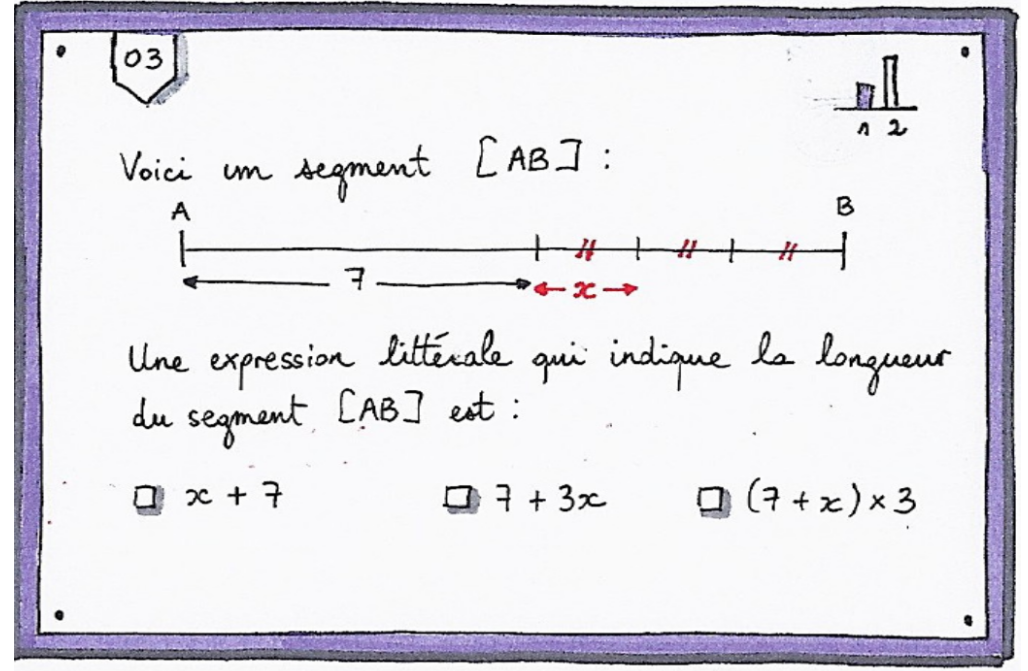
\includegraphics[width=\linewidth]{Images/CalculLitteral1.png}
            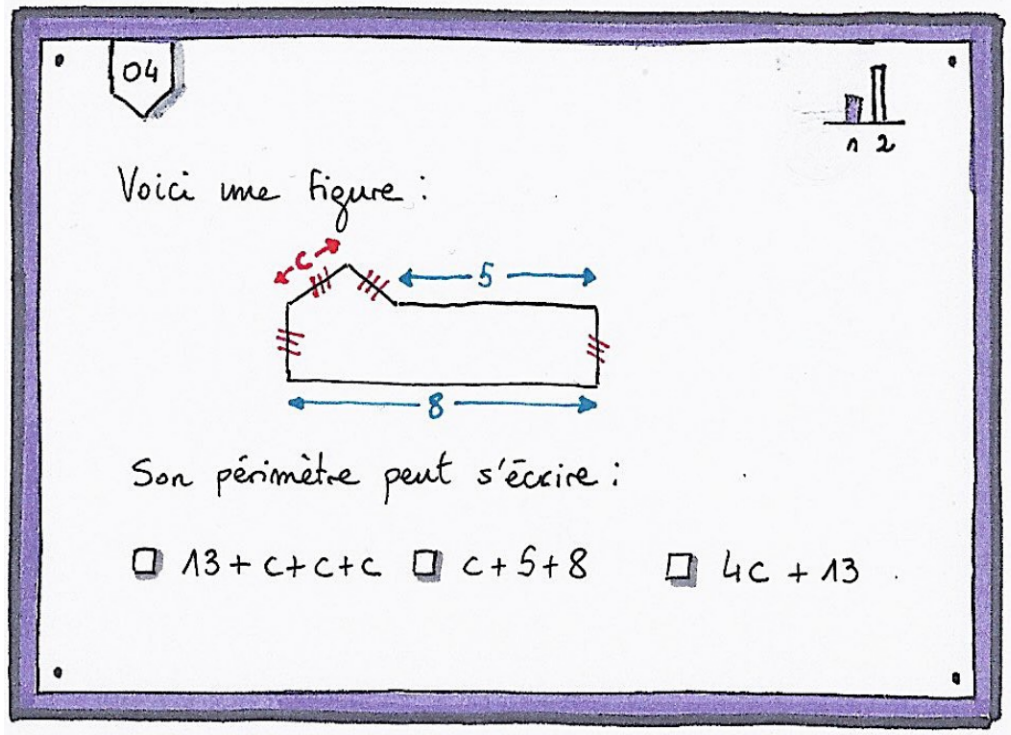
\includegraphics[width=\linewidth]{Images/CalculLitteral2.png}
            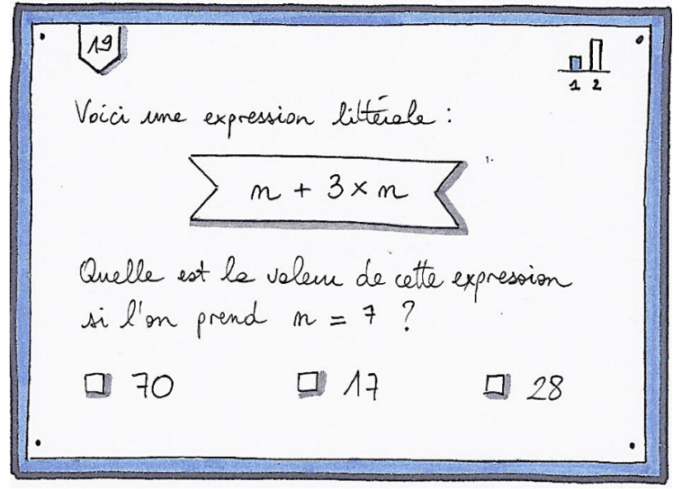
\includegraphics[width=\linewidth]{Images/CalculLitteral3.png}
        \end{exercice}

        \begin{exercice}
            \begin{center}
                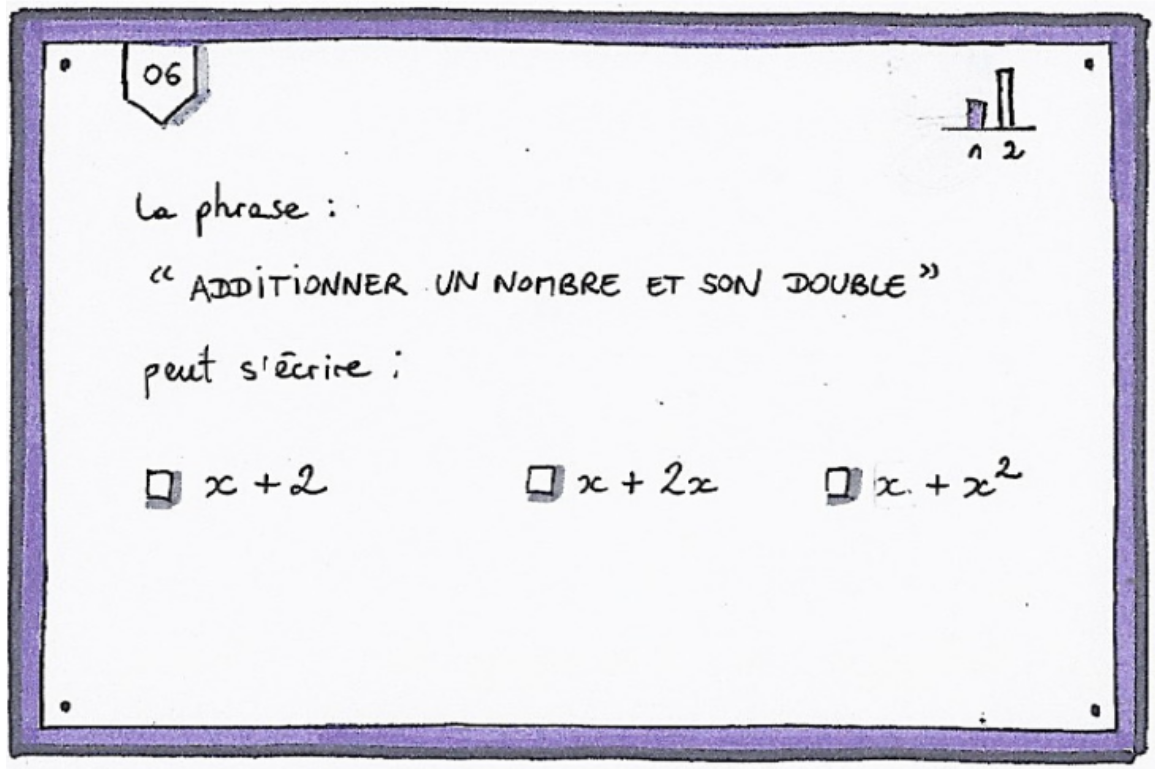
\includegraphics[width=0.95\linewidth]{Images/CalculLitteral4.png}
            \end{center}
        \end{exercice}

        \begin{exercice}[Titre=En fonction de …]
            Exprimer en fonction du nombre $n$ :
            \begin{enumerate}
                \item Le triple de $n$.
                \item Le double de $n$.
                \item La moitié de $n$.
                \item Le périmètre d’un carré de côté $n$.
                \item L’aire d’un carré de côté $n$.
            \end{enumerate}
        \end{exercice}

        \begin{exercice}
            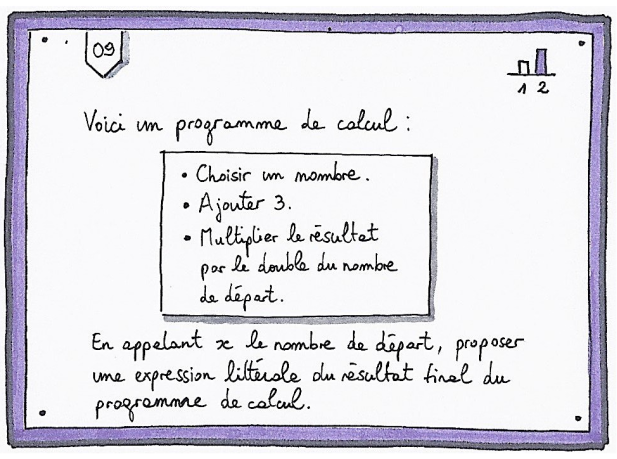
\includegraphics[width=\linewidth]{Images/CalculLitteral5.png}
        \end{exercice}

        \begin{exercice}
            Calcule la valeur de l’expression littérale
            \[
                \textrm{A} = 5 n - 12
            \]
            lorsque :
            \begin{enumerate}
                \item $n=11$
                \item $n=4$
                \item $n=1$
                \item $n=2,4$
            \end{enumerate}
        \end{exercice}

        \begin{exercice}
            Calcule la valeur de l’expression littérale
            \[
                \textrm{B} = \dfrac{x+1}{2} - 10
            \]
            lorsque :
            \begin{enumerate}
                \item $x=63$
                \item $x=40$
                \item $x=24$
                \item $x=7$
            \end{enumerate}

            Es-tu capable de trouver une valeur de $x$ pour laquelle $\textrm{B}=0$?
        \end{exercice}

        \columnbreak

        \begin{exercice}
            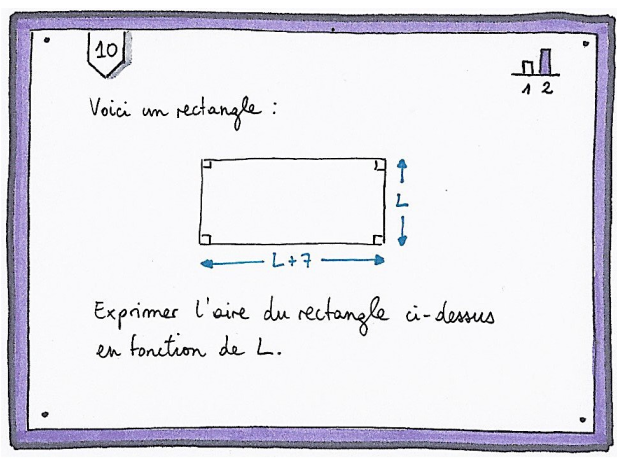
\includegraphics[width=\linewidth]{Images/CalculLitteral6.png}
            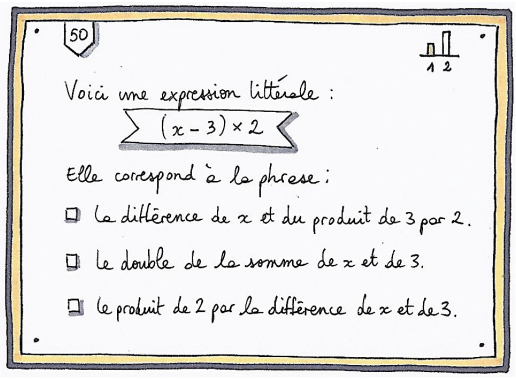
\includegraphics[width=\linewidth]{Images/CalculLitteral7.png}
        \end{exercice}

        \begin{exercice}
            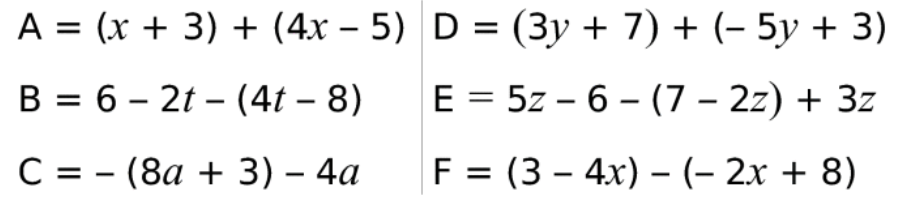
\includegraphics[width=\linewidth]{Images/CalculLitteral8.png}
            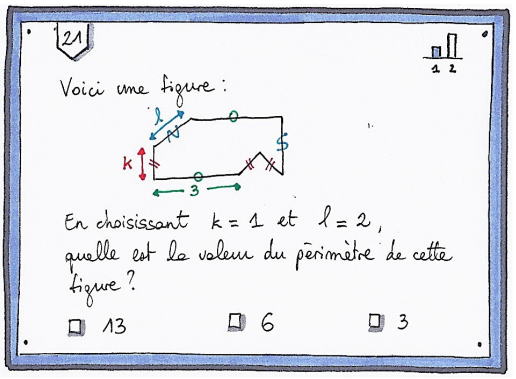
\includegraphics[width=\linewidth]{Images/CalculLitteral9.png}
        \end{exercice}

        \begin{exercice}
            Réduire les exepressions suivantes.
            \begin{multicols}{2}
                \begin{enumerate}[label=\textbf{\alph*.}]
                    \item $6\times x$
                    \item $x \times 7$
                    \item $y \times 1$
                    \item $0 \times t$
                    \item $u \times u$
                    \item $6\times a \times 2$
                    \item $a \times 3 \times b$
                    \item $4\times x \times 10\times y$
                    \item $2\times x \times 4 \times x$
                    \item $2x\times 5$
                    \item $3a \times 2a$
                    \item $w \times v \times w$
                    \item $2c \times 5d$
                    \item $e \times 3f \times e$
                \end{enumerate}
            \end{multicols}
        \end{exercice}

        \begin{exercice}
            Réduire les exepressions suivantes.\\
            \emph{Recopier chaque expression et souligner de couleurs différentes les termes de « familles » différentes.}
            \begin{enumerate}[label=\textbf{\alph*.}]
                \item $6x + 2x$
                \item $6x + 2$
                \item $3a + 2 + 5a$
                \item $20y - 5 -2y$
                \item $5a + 10b - 2a + 3b$
                \item $3x -2 -2x + 10$
                \item $s + 9t + s - 10t$
                \item $5x^2 + 10x - 2x^2 + 4 - x + 1$
            \end{enumerate}
        \end{exercice}

        \begin{exercice}
            Réduire les exepressions suivantes.\\
            \emph{Recopier chaque expression, souligner les produits prioritaires, les réduire puis terminer en réduisant les sommes et différences.}
            \begin{enumerate}[label=\textbf{\alph*.}]
                \item $6 + 2 \times x$
                \item $4 \times s + s \times 5 - 3$
                \item $-10 + 3 \times s + 2 \times 2$
                \item $y \times 5 + 3 - 2 \times y$
                \item $3 - 3 \times x + x \times 5$
                \item $4 \times 4 - 4 \times y - 4$
                \item $5 \times 3 + 2 \times d - 4$
                \item $5 + 3 \times e - 2 \times 3$
                \item $3 \times m - 3 \times m + 4$
                \item $8 \times h - 10 - h \times 7$
                \item $3 \times i + 4 \times 2 - i \times 2$
            \end{enumerate}
        \end{exercice}

        \newpage

        \begin{exercice}
            Recopier chaque expression, supprimer les parenthèses et réduire.\\
            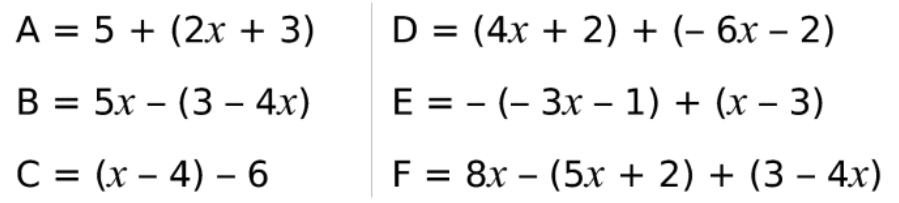
\includegraphics[width=\linewidth]{Images/Parenthèses1.png}
        \end{exercice}

        \begin{exercice}
            Même consigne.\\
            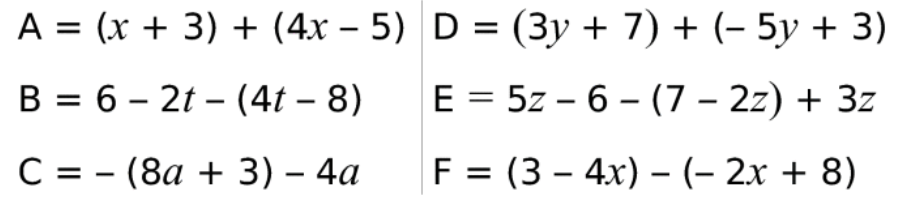
\includegraphics[width=\linewidth]{Images/Parenthèses2.png}
        \end{exercice}
        \columnbreak
        \begin{exercice}
            Recopier chaque pyramide puis détailler sur ton cahier les calculs nécessaires pour compléter les cases vides en respectant les règles indiquées à droite.\\
            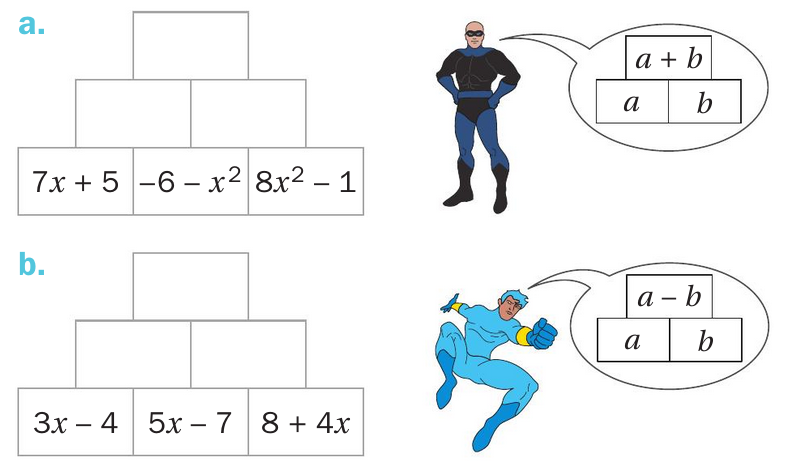
\includegraphics[width=\linewidth]{Images/Pyramides.png}
        \end{exercice}

    \end{Maquette}

\end{multicols}

\end{document}
